\documentclass[12pt]{article}
\usepackage[utf8]{inputenc}
\usepackage{amsmath}
\usepackage{fancyhdr}
\usepackage{graphicx}
\usepackage{epstopdf}

\setlength{\oddsidemargin}{0in}
\setlength{\evensidemargin}{0in}
\setlength{\textwidth}{6.5in}
\setlength{\topmargin}{-.3in}
\setlength{\textheight}{9in}


\pagestyle{fancy}
\begin{document}

\begin{center}
{\Large Machine Learnig Homework 7} \\[.3in]
\end{center}
\lhead{Adam Kosiorek}
\rhead{IMAT: 03661883}
\vspace*{.5in}

\section*{Problem 1}
If the data set is linearly separable, any decision boundary separating the two classes will have the property
\begin{equation}
w^T\phi(x^n) = \begin{cases} \geq 0 & \mbox{if } z^n = 1, \\ < 0 & otherwise. \\ \end{cases}
\label{eq:}
\end{equation}

Moreover, the log-likelihood 
\begin{align}
L(w) &= \log p(\{z^i\}|w,\{\phi(x^i)\})\\
&= \sum^{N}_{n = 1}\left[z^n\log \sigma(w^T\phi(x^n)) + (1-z^n)(\log(1-\sigma(w^T\phi(x^n))))\right]
\end{align}

will be maximized when $y^n = \sigma(w^T\phi(x^n)) = z^n \hspace{0.3cm}\forall n$. This will be the case when the sigmoid function is saturated, which occurs when its argument, $w^T\phi$, goes to $\pm \inf$, i.e., when the magnitude of $w$ goes to infinity. 


\section*{Problem 2}
The basis function 
\begin{equation}
\phi(x_1,x_2) = x_1x_2
\end{equation}

enables us to linearly seperate the crosses from the circles. The hyperplane would go through the origin of the coordinate system.

\section*{Problem 5}

Let $\mathbf{w}^0 = \mathbf{0}$ be an initial set of weights and $b^0 = 0$ an initial bias. Let $z_k^i \in \{-1, 1\}$ denote the classification result of the $i^{th}$ training sample $\mathbf{x}^i$, $i = 1, \ldots, N$ using weights $\mathbf{w}^k$ and bias $b^k$. The training algorithm iterates as long as there is at least one misclassification and computes:
\begin{equation}
\begin{align}
  \mathbf{w}^{k+1} &= \mathbf{w}^k + \sum_{t^i \neq z_k^i} t^i \mathbf{x}^i \\
  b^{k+1} &= b^k + \sum_{t^i \neq z_k^i} t^i
\end{align}
\label{eq:train}
\end{equation}

\section*{Problem 6}

\begin{figure}[!ht]
 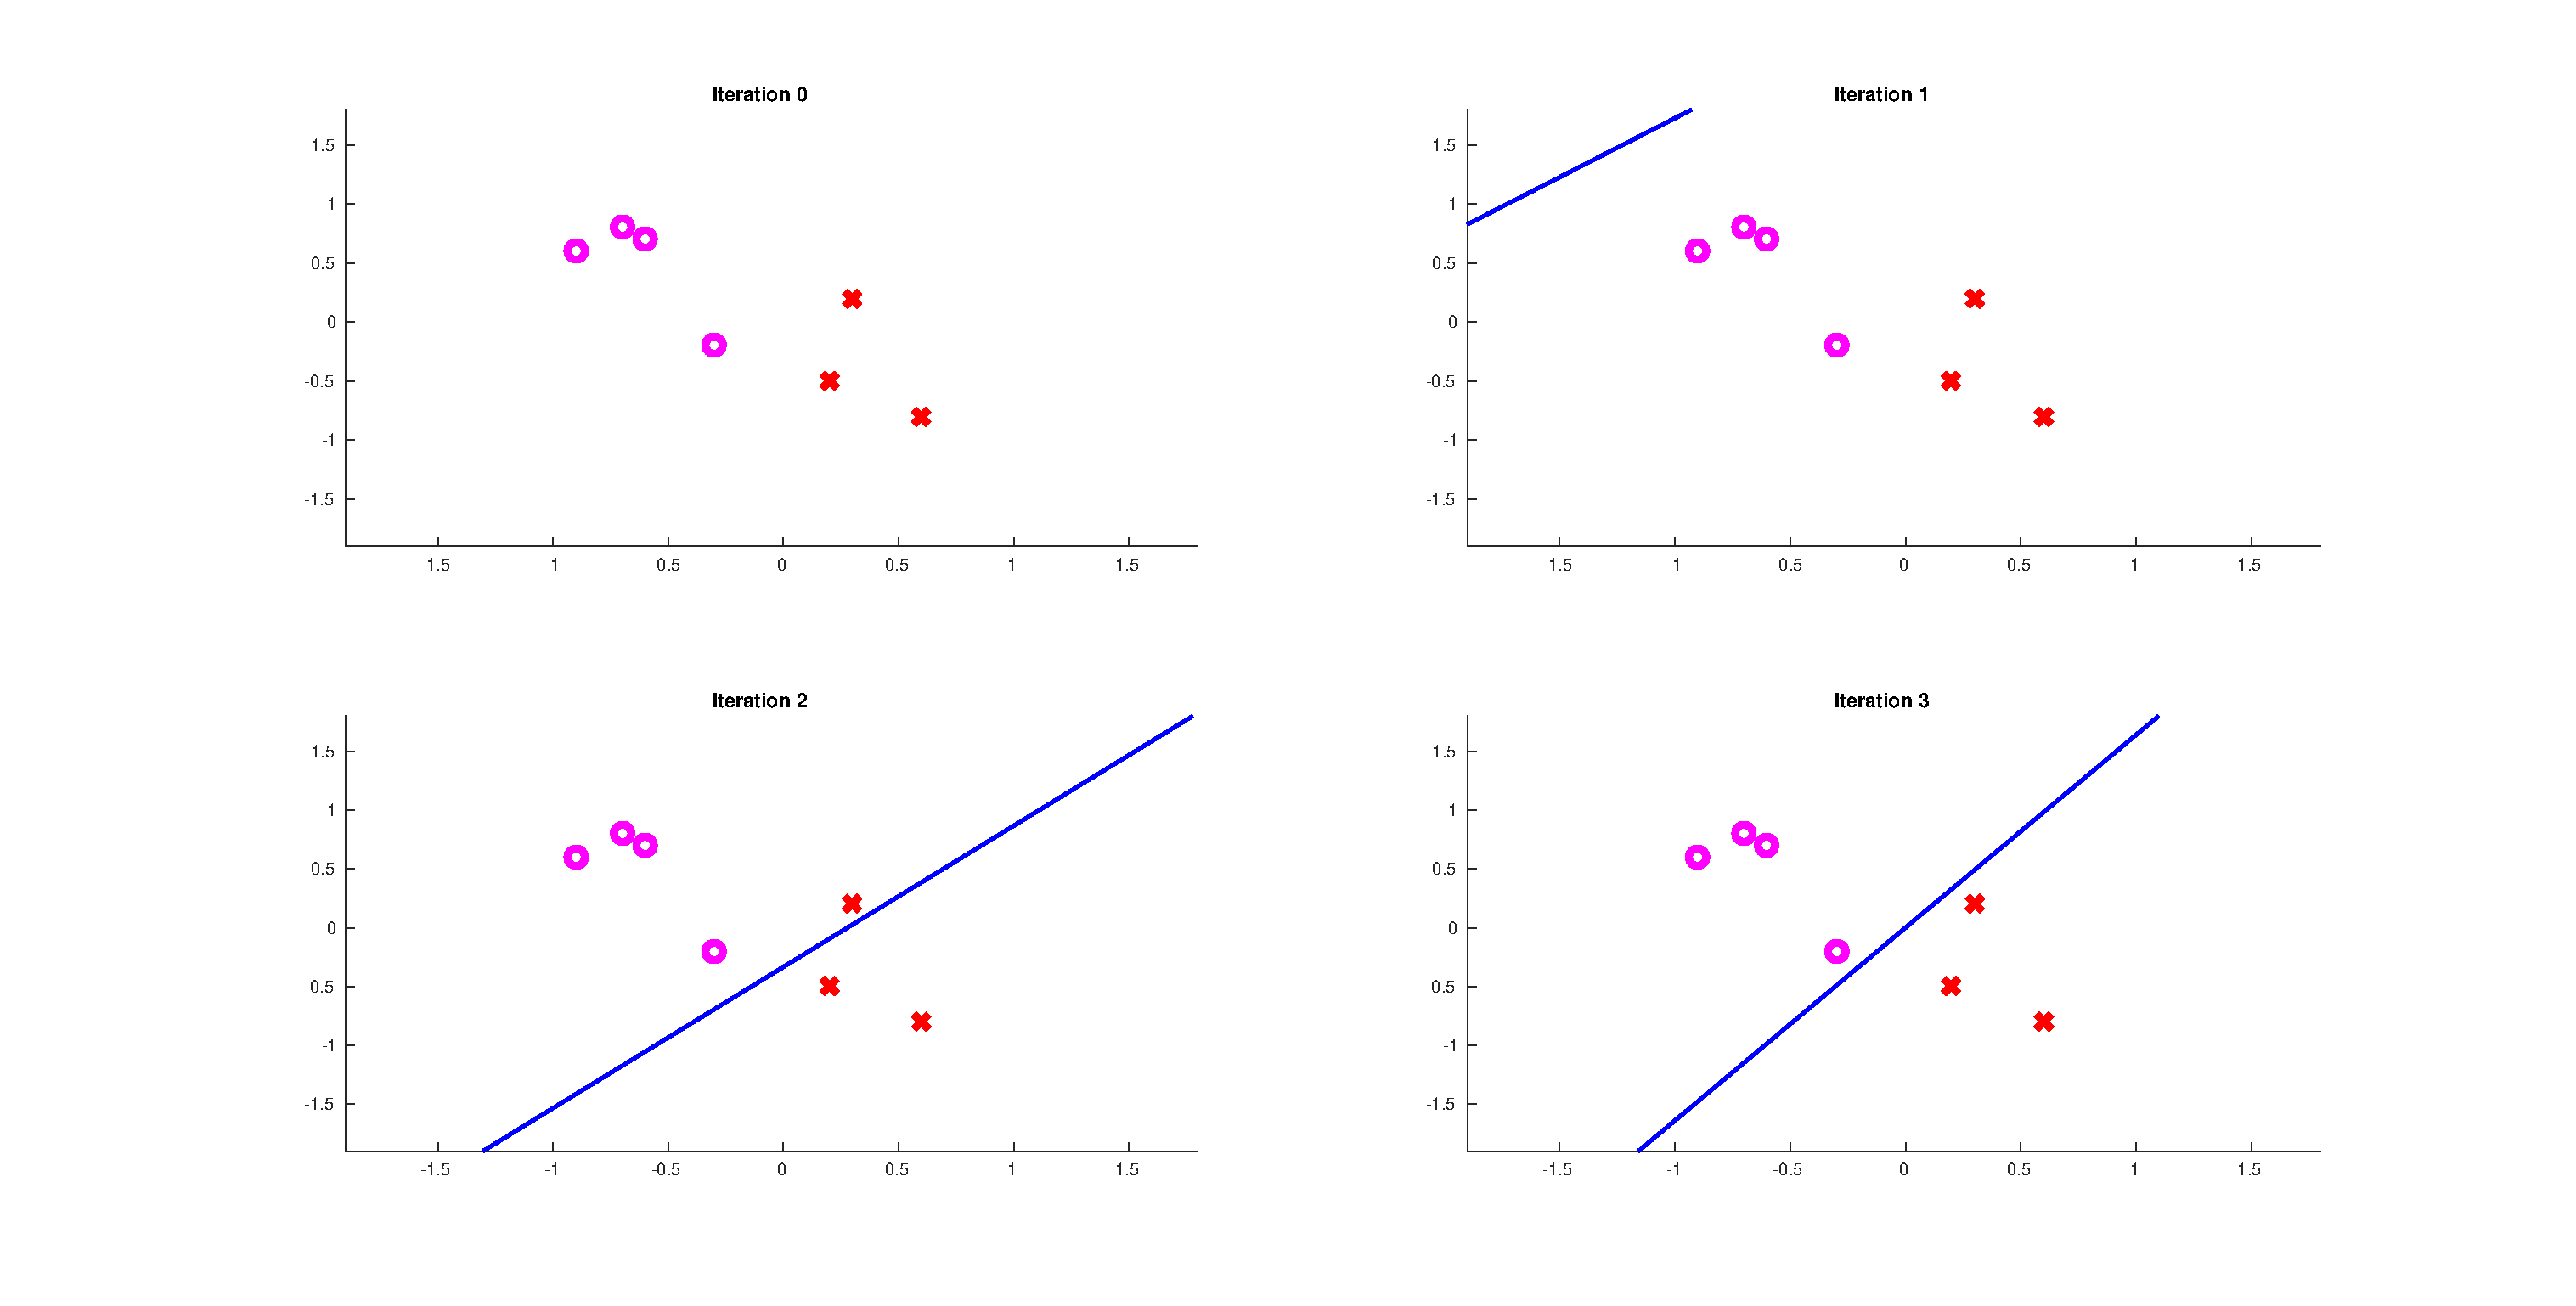
\includegraphics[width=\textwidth]{perceptron6}
 \caption{Decision boundary after 0-3 iterations.}
 \label{fig:prob6}
\end{figure}

Figure \ref{fig:prob6} shows the decision boundary after 0-3 training iterations. After the third iteration it does not change anymore; The norm of the weights $||\mathbf{w}^k||$ grows to infinity, however.


\section*{Problem 7}

Let $z_k^i \in \{-1, 1\}$ denote the classification result of the $i^{th}$ training sample $\mathbf{x}^i$, $i = 1, \ldots, N$. Since $\mathbf{x}^i$ are linearly separable, it holds that $ \mathbf{x}^i > 0 \implies t^i \widetilde{\mathbf{w}}^T \mathbf{x}^i > 0$. If we define $\gamma = \min\limits_{\mathbf{x}^i} t^i \widetilde{\mathbf{w}}^T \mathbf{x}^i$ then:

\begin{equation}
 \widetilde{\mathbf{w}}^T \mathbf{w}^k = \widetilde{\mathbf{w}}^T \mathbf{w}^{k-1} + \sum_{t^i \neq z_{k-1}^i} t^i \widetilde{\mathbf{w}}^T \mathbf{x}^i \geq \widetilde{\mathbf{w}}^T \mathbf{w}^{k-1} + \gamma \geq \widetilde{\mathbf{w}}^T \mathbf{w}^{0} + k \gamma = k \gamma
\end{equation}


\section*{Problem 8}

From equation \ref{eq:train} and since $||\mathbf{x}^i|| < R$ and the number of misclassified samples at each iteration is at most $N$ we have

\begin{equation}
 \begin{align}
  ||\mathbf{w}^k||^2 &\leq ||\mathbf{w}^{k-1}||^2 + \sum_{t^i \neq z_{k-1}^i} ||\mathbf{x}^i||^2 \\
		     &\leq ||\mathbf{w}^{k-1}||^2 + \sum_{t^i \neq z_{k-1}^i} R^2 \\
		     &\leq ||\mathbf{w}^{k-1}||^2 + N R^2 \\
		     &\leq k N R^2 \\
 \end{align}
\end{equation}

\section*{Problem 9}
  From problems 7 and 8 we know that $||\widetilde{\mathbf{w}}^T \mathbf{w}^k|| \geq k \gamma$ and $||\mathbf{w}^k||^2 < k R^2$. Therefore:

\begin{equation}
 \frac{k^2 \gamma^2}{k R^2} = \frac{k \gamma^2}{R^2} \leq \frac{\left( \widetilde{\mathbf{w}}^T \mathbf{w}^k \right)^2}{||\mathbf{w}^k||^2}
\end{equation}

Since $\left( \widetilde{\mathbf{w}}^T \mathbf{w}^k \right)^2 = \sum_i \widetilde{\mathbf{w}}_i^2 (\mathbf{w}^k)_i^2 = \sum_i \widetilde{\mathbf{w}}_i^2 \sum_i (\mathbf{w}^k)_i^2 = ||\widetilde{\mathbf{w}}||^2 ||\mathbf{w}^k||^2$ and

\begin{equation}
 \frac{k \gamma^2}{R^2} \leq \||\widetilde{\mathbf{w}}||^2
\end{equation}

\begin{equation}
 k \leq \frac{||\widetilde{R^2 \mathbf{w}}||^2}{\gamma^2}
\end{equation}


  
\end{document}
